\documentclass[]{report}
\usepackage{lmodern}
\usepackage{amssymb,amsmath}
\usepackage{ifxetex,ifluatex}
\usepackage{fixltx2e} % provides \textsubscript
\ifnum 0\ifxetex 1\fi\ifluatex 1\fi=0 % if pdftex
  \usepackage[T1]{fontenc}
  \usepackage[utf8]{inputenc}
\else % if luatex or xelatex
  \ifxetex
    \usepackage{mathspec}
  \else
    \usepackage{fontspec}
  \fi
  \defaultfontfeatures{Ligatures=TeX,Scale=MatchLowercase}
\fi
% use upquote if available, for straight quotes in verbatim environments
\IfFileExists{upquote.sty}{\usepackage{upquote}}{}
% use microtype if available
\IfFileExists{microtype.sty}{%
\usepackage{microtype}
\UseMicrotypeSet[protrusion]{basicmath} % disable protrusion for tt fonts
}{}
\usepackage[margin=1in]{geometry}
\usepackage{hyperref}
\hypersetup{unicode=true,
            pdftitle={Informe prototipo},
            pdfauthor={SmartCrop},
            pdfborder={0 0 0},
            breaklinks=true}
\urlstyle{same}  % don't use monospace font for urls
\usepackage{natbib}
\bibliographystyle{apalike}
\usepackage{longtable,booktabs}
\usepackage{graphicx,grffile}
\makeatletter
\def\maxwidth{\ifdim\Gin@nat@width>\linewidth\linewidth\else\Gin@nat@width\fi}
\def\maxheight{\ifdim\Gin@nat@height>\textheight\textheight\else\Gin@nat@height\fi}
\makeatother
% Scale images if necessary, so that they will not overflow the page
% margins by default, and it is still possible to overwrite the defaults
% using explicit options in \includegraphics[width, height, ...]{}
\setkeys{Gin}{width=\maxwidth,height=\maxheight,keepaspectratio}
\IfFileExists{parskip.sty}{%
\usepackage{parskip}
}{% else
\setlength{\parindent}{0pt}
\setlength{\parskip}{6pt plus 2pt minus 1pt}
}
\setlength{\emergencystretch}{3em}  % prevent overfull lines
\providecommand{\tightlist}{%
  \setlength{\itemsep}{0pt}\setlength{\parskip}{0pt}}
\setcounter{secnumdepth}{5}
% Redefines (sub)paragraphs to behave more like sections
\ifx\paragraph\undefined\else
\let\oldparagraph\paragraph
\renewcommand{\paragraph}[1]{\oldparagraph{#1}\mbox{}}
\fi
\ifx\subparagraph\undefined\else
\let\oldsubparagraph\subparagraph
\renewcommand{\subparagraph}[1]{\oldsubparagraph{#1}\mbox{}}
\fi

%%% Use protect on footnotes to avoid problems with footnotes in titles
\let\rmarkdownfootnote\footnote%
\def\footnote{\protect\rmarkdownfootnote}

%%% Change title format to be more compact
\usepackage{titling}

% Create subtitle command for use in maketitle
\newcommand{\subtitle}[1]{
  \posttitle{
    \begin{center}\large#1\end{center}
    }
}

\setlength{\droptitle}{-2em}
  \title{Informe prototipo}
  \pretitle{\vspace{\droptitle}\centering\huge}
  \posttitle{\par}
  \author{SmartCrop}
  \preauthor{\centering\large\emph}
  \postauthor{\par}
  \predate{\centering\large\emph}
  \postdate{\par}
  \date{2017-05-01}

\usepackage{booktabs}
\usepackage{amsthm}
\makeatletter
\def\thm@space@setup{%
  \thm@preskip=8pt plus 2pt minus 4pt
  \thm@postskip=\thm@preskip
}
\makeatother

\begin{document}
\maketitle

{
\setcounter{tocdepth}{1}
\tableofcontents
}
\chapter{Resumen}\label{resumen}

Este documento corresponde a un informe prototipo de análisis
vegetacional realizado en base a información satelital para una fecha
puntual como soporte a la toma de decisiones para los agricultores. La
fecha de captura de la imágenes satelitales fué el \textbf{29 de enero
2017}. En este prototipo se consideraron seis predios ubicados en la
comuna de San Carlos correspondientes a cultivos de maiz y cerezos. El
informe esta estructurado con las secciones:

\begin{enumerate}
\def\labelenumi{\arabic{enumi}.}
\tightlist
\item
  \protect\hyperlink{DescripcionVIs}{Descripción índices vegetacionales}
\item
  \protect\hyperlink{DescipcionVIs}{Composición de imágenes}
\item
  \protect\hyperlink{indicesVeg}{Índices vegetacionales}
\item
  \protect\hyperlink{AnalisisDatos}{Análisis de datos}
\end{enumerate}

\hypertarget{DescripcionVIs}{\chapter{Descripción Índices
Vegetacionales}\label{DescripcionVIs}}

En esta sección se describen las principales caracteristicas de los
índices usados para el monitoreo del estado vegetacional de lso
cultivos.

\begin{enumerate}
\def\labelenumi{\arabic{enumi}.}
\item
  \textbf{Relación simple (SR):} Well known and often used index,
  described as the ratio of light that is scattered in the near
  infra-red range to that which is absorbed in the red range. Values
  description: The range of values is from 0 to more than 30, where
  healthy vegetation generally falls between values of 2 to 8.
\item
  \textbf{Índice de Vegetación ajustado al Suelo (SAVI):}
\item
  \textbf{Borde Rojo - Índice Normalizado de Diferencia de Agua
  (RE-NDWI:}
\item
  \textbf{Borde Rojo - Índice Normalizado de Diferencia de Vegetación
  (RE-NDVI):}
\end{enumerate}

\chapter{Composición de imágenes}\label{compoIma}

En esta sección se presenta la composición de imagenes de color
verdadero junto con 3 composiciones que permiten resaltar
caracteristicas de la vegetación.

\section{Fundo Rondadero}\label{fundo-rondadero}

\begin{figure}

{\centering 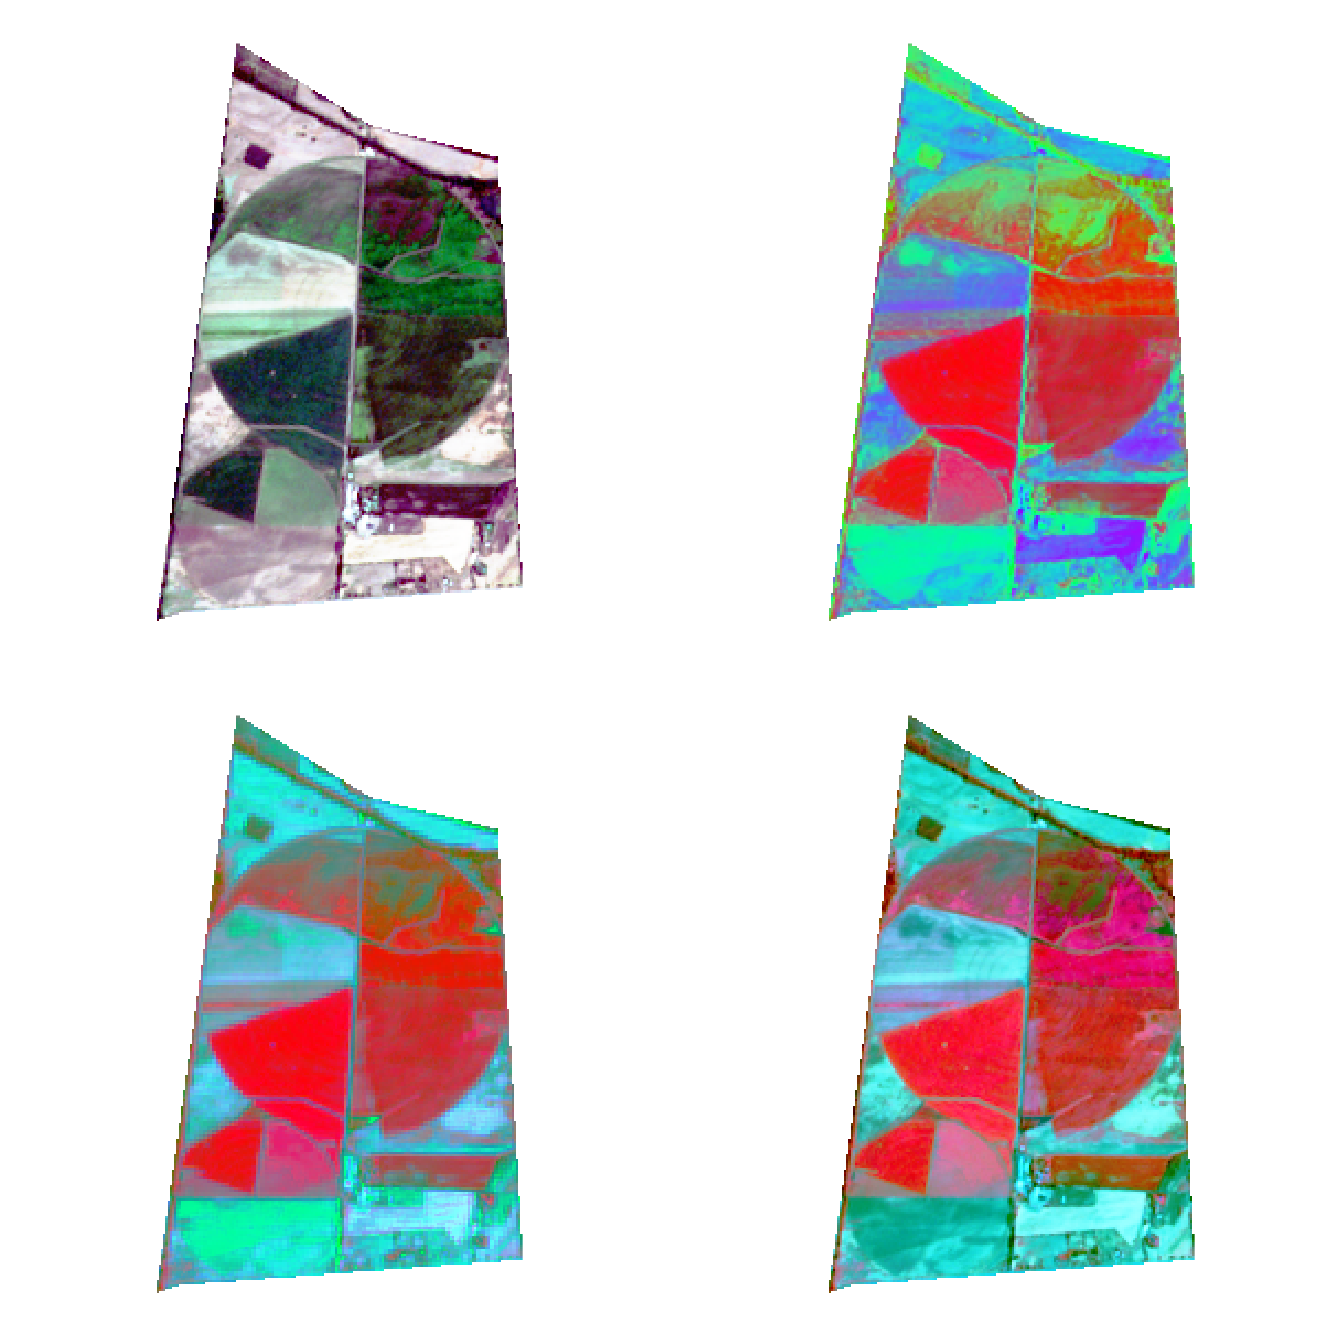
\includegraphics[width=1\linewidth]{bookdown-demo_files/figure-latex/nice-fig-1} 

}

\caption[one plot]{Composición de color}\label{fig:nice-fig}
\end{figure}

\section{Predios Fernando Rueda}\label{predios-fernando-rueda}

\subsection{Predio 1}\label{predio-1}

\begin{figure}

{\centering 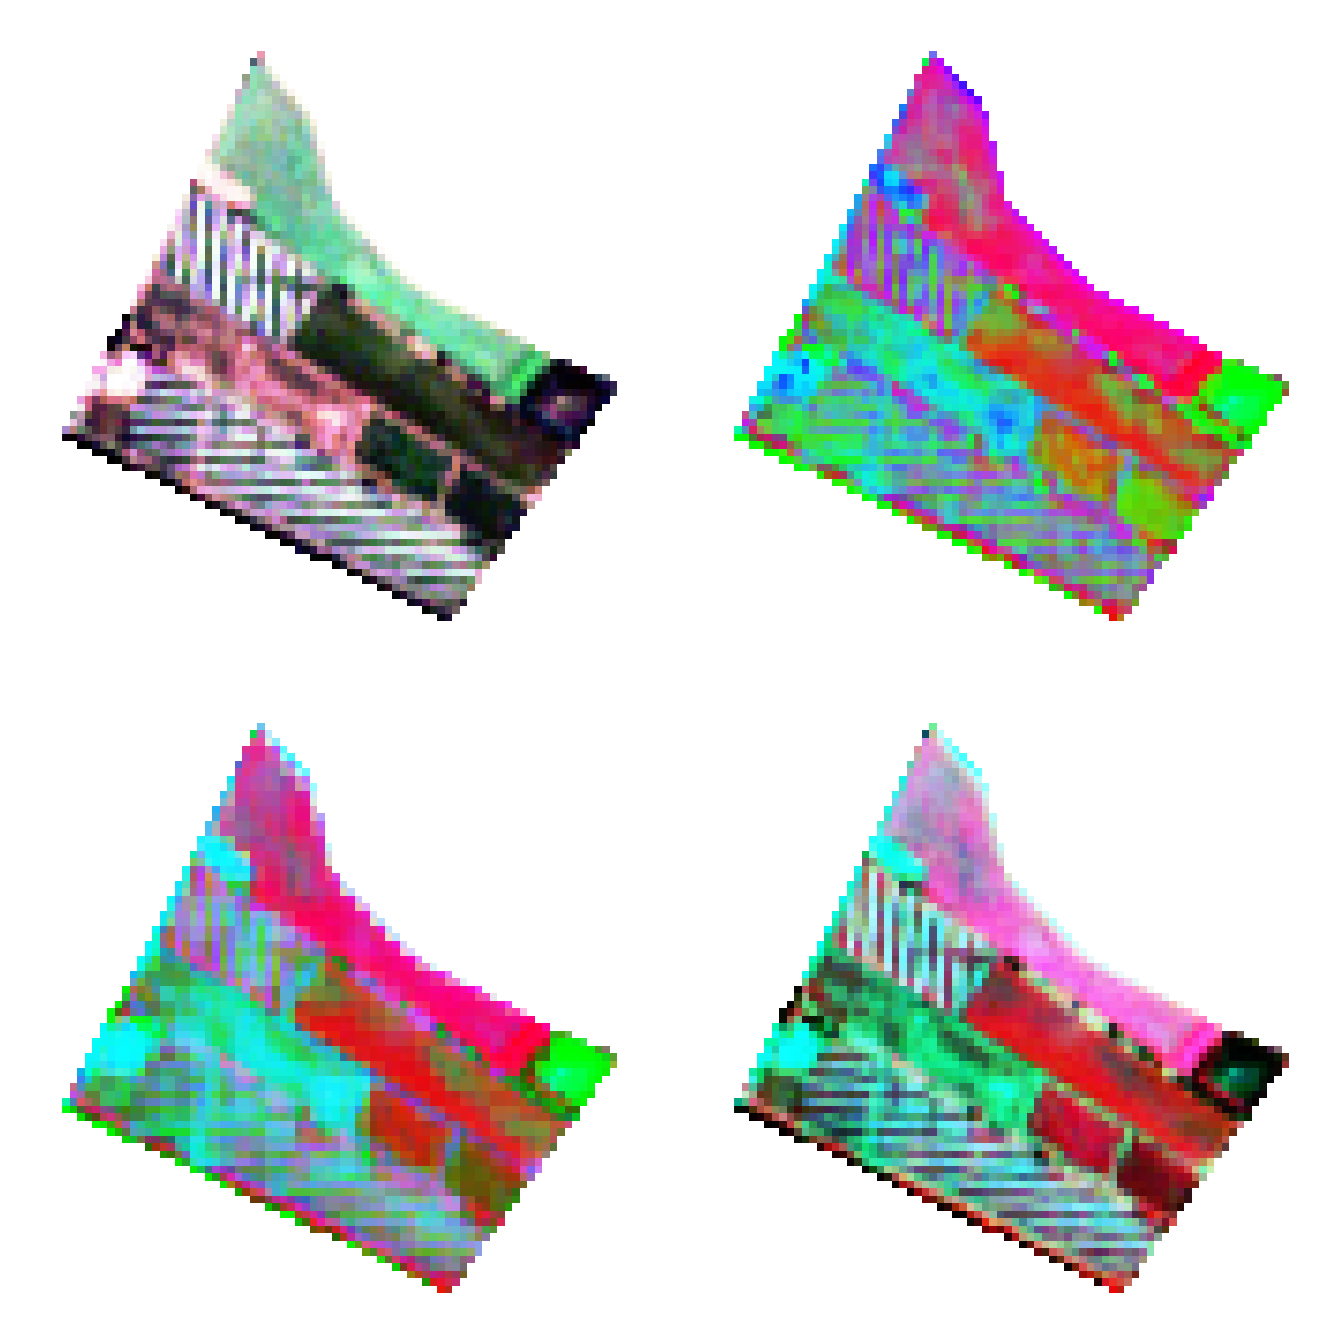
\includegraphics[width=1\linewidth]{bookdown-demo_files/figure-latex/nice-fig2-1} 

}

\caption[one plot]{Composición de color}\label{fig:nice-fig2}
\end{figure}

\subsection{Predio 2}\label{predio-2}

\begin{figure}

{\centering 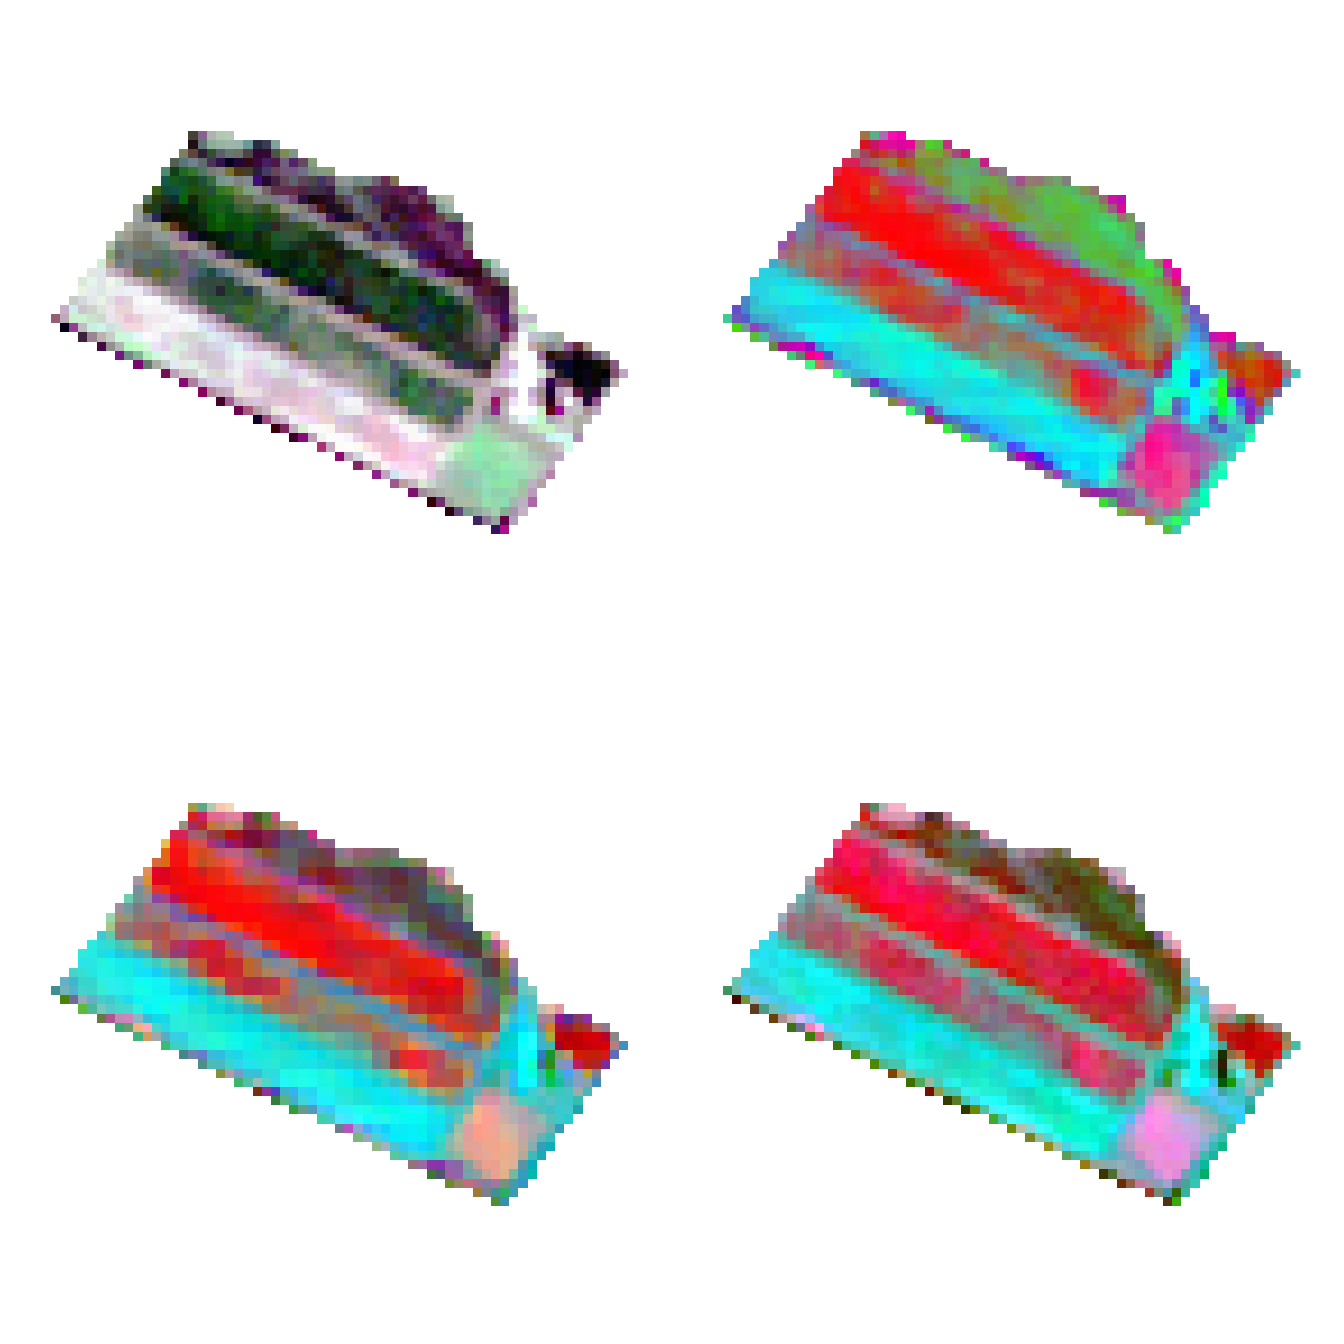
\includegraphics[width=1\linewidth]{bookdown-demo_files/figure-latex/nice-fig3-1} 

}

\caption[one plot]{Composición de color}\label{fig:nice-fig3}
\end{figure}

\subsection{Predio 3}\label{predio-3}

\begin{figure}

{\centering 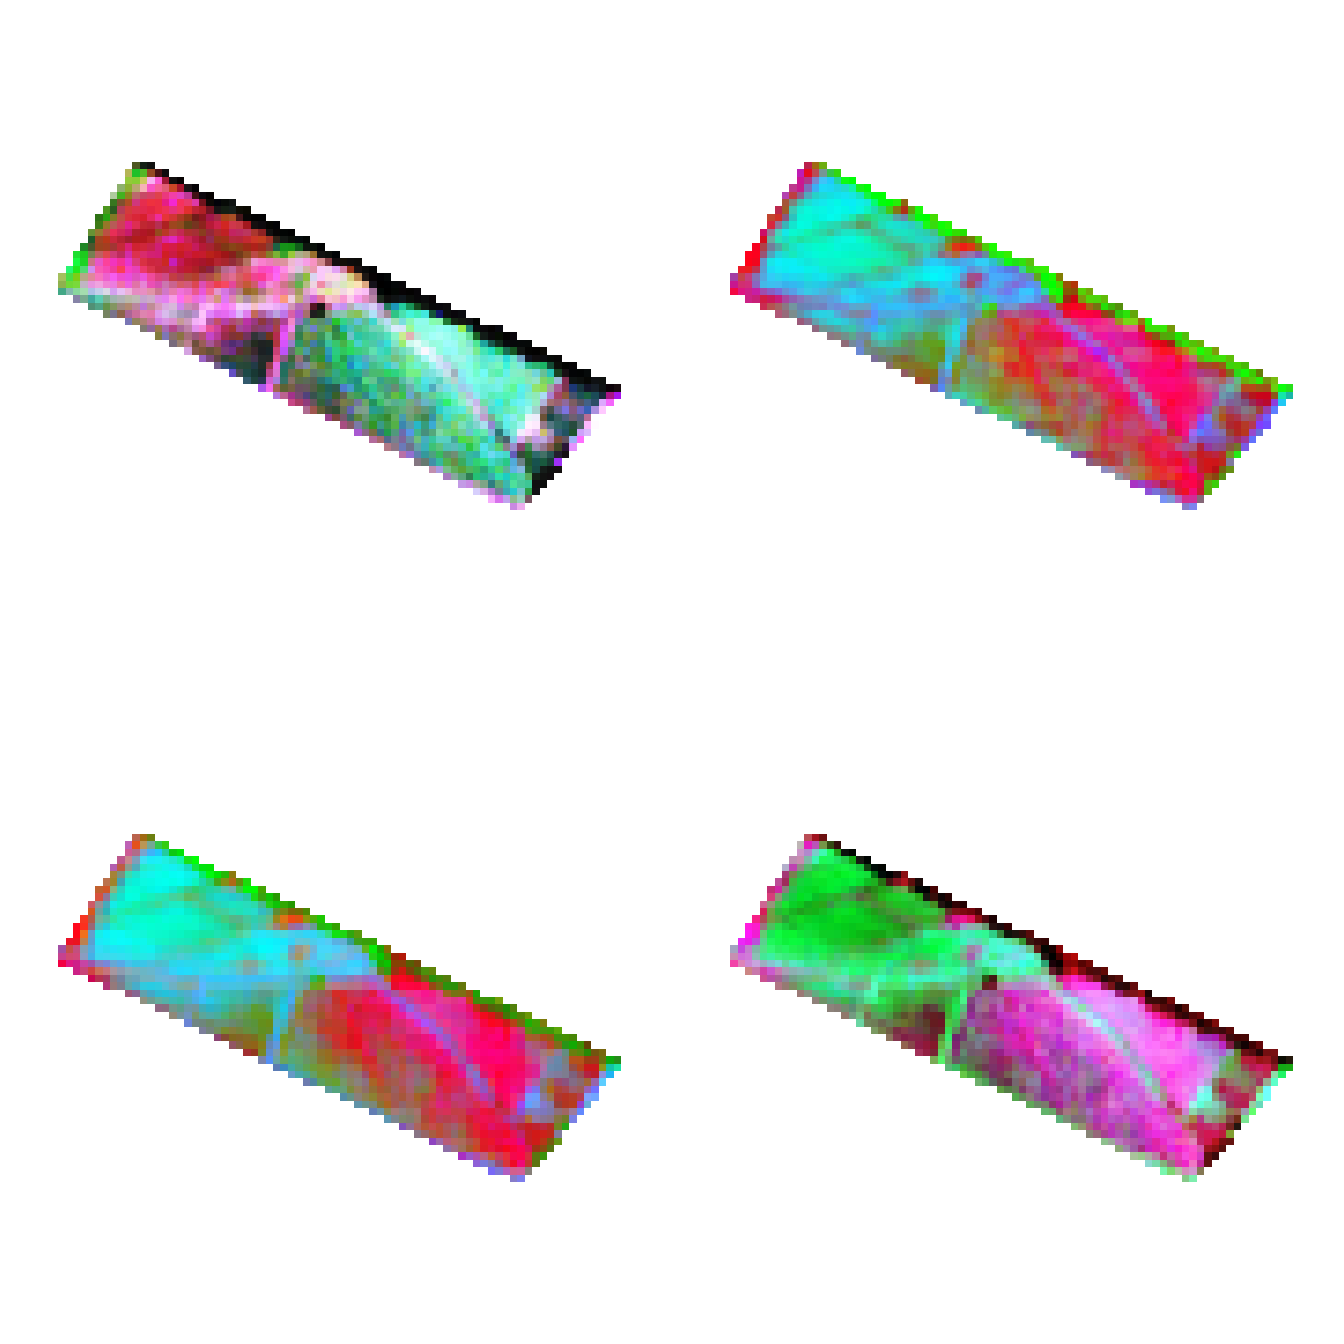
\includegraphics[width=1\linewidth]{bookdown-demo_files/figure-latex/nice-fig4-1} 

}

\caption[one plot]{Composición de color}\label{fig:nice-fig4}
\end{figure}

\subsection{Predio 4}\label{predio-4}

\begin{figure}

{\centering 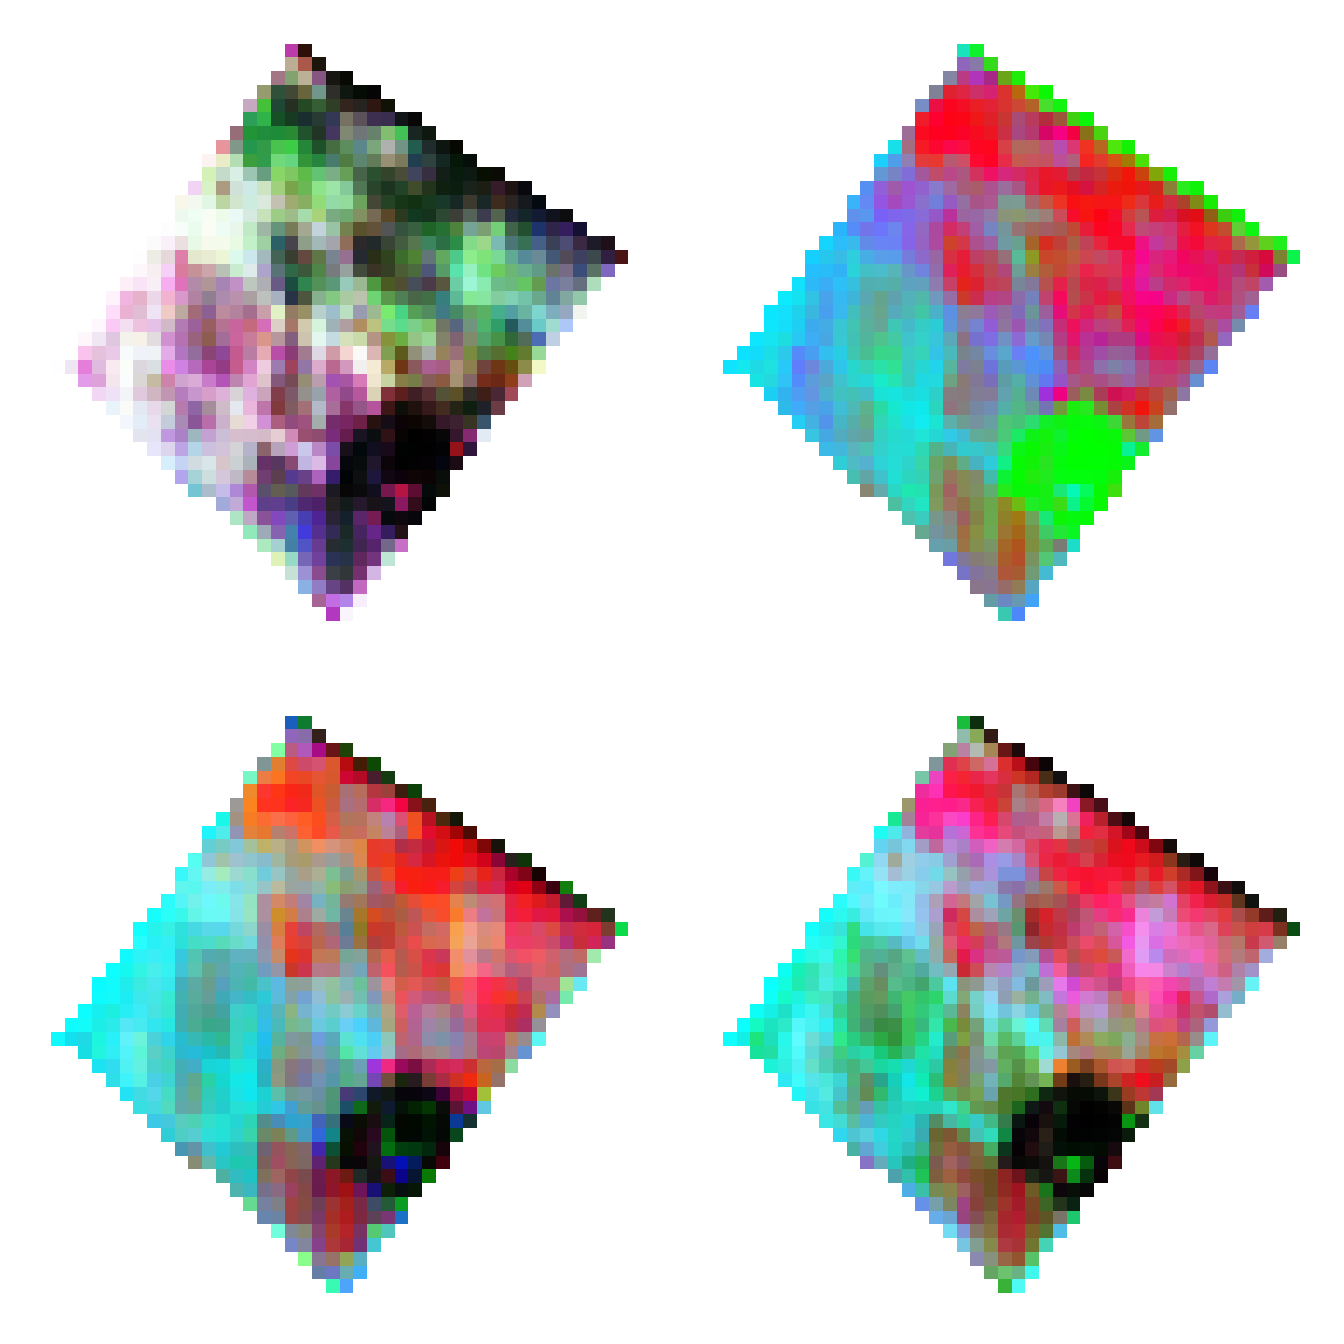
\includegraphics[width=1\linewidth]{bookdown-demo_files/figure-latex/nice-fig5-1} 

}

\caption[one plot]{Composición de color}\label{fig:nice-fig5}
\end{figure}

\subsection{Predio 5}\label{predio-5}

\begin{figure}

{\centering 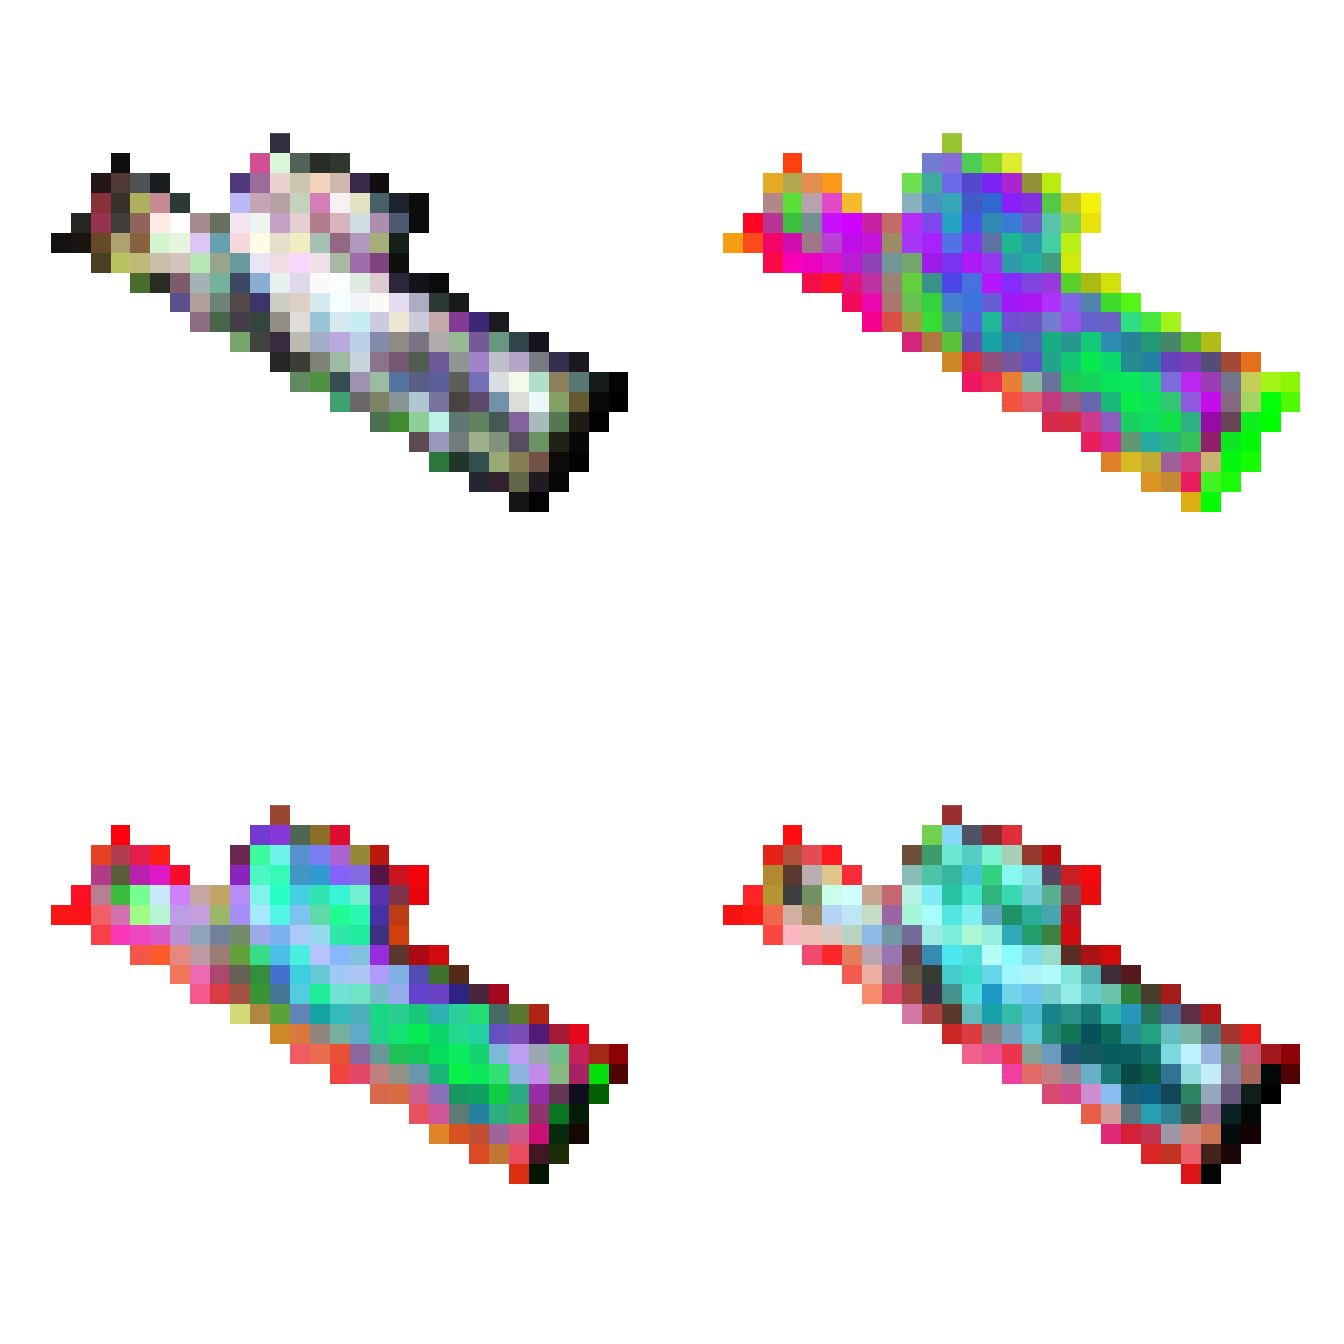
\includegraphics[width=1\linewidth]{bookdown-demo_files/figure-latex/nice-fig6-1} 

}

\caption[one plot]{Composición de color}\label{fig:nice-fig6}
\end{figure}

\hypertarget{indicesVeg}{\chapter{Índices
vegetacionales}\label{indicesVeg}}

\section{Fundo Rondadero}\label{fundo-rondadero-1}

\begin{figure}

{\centering 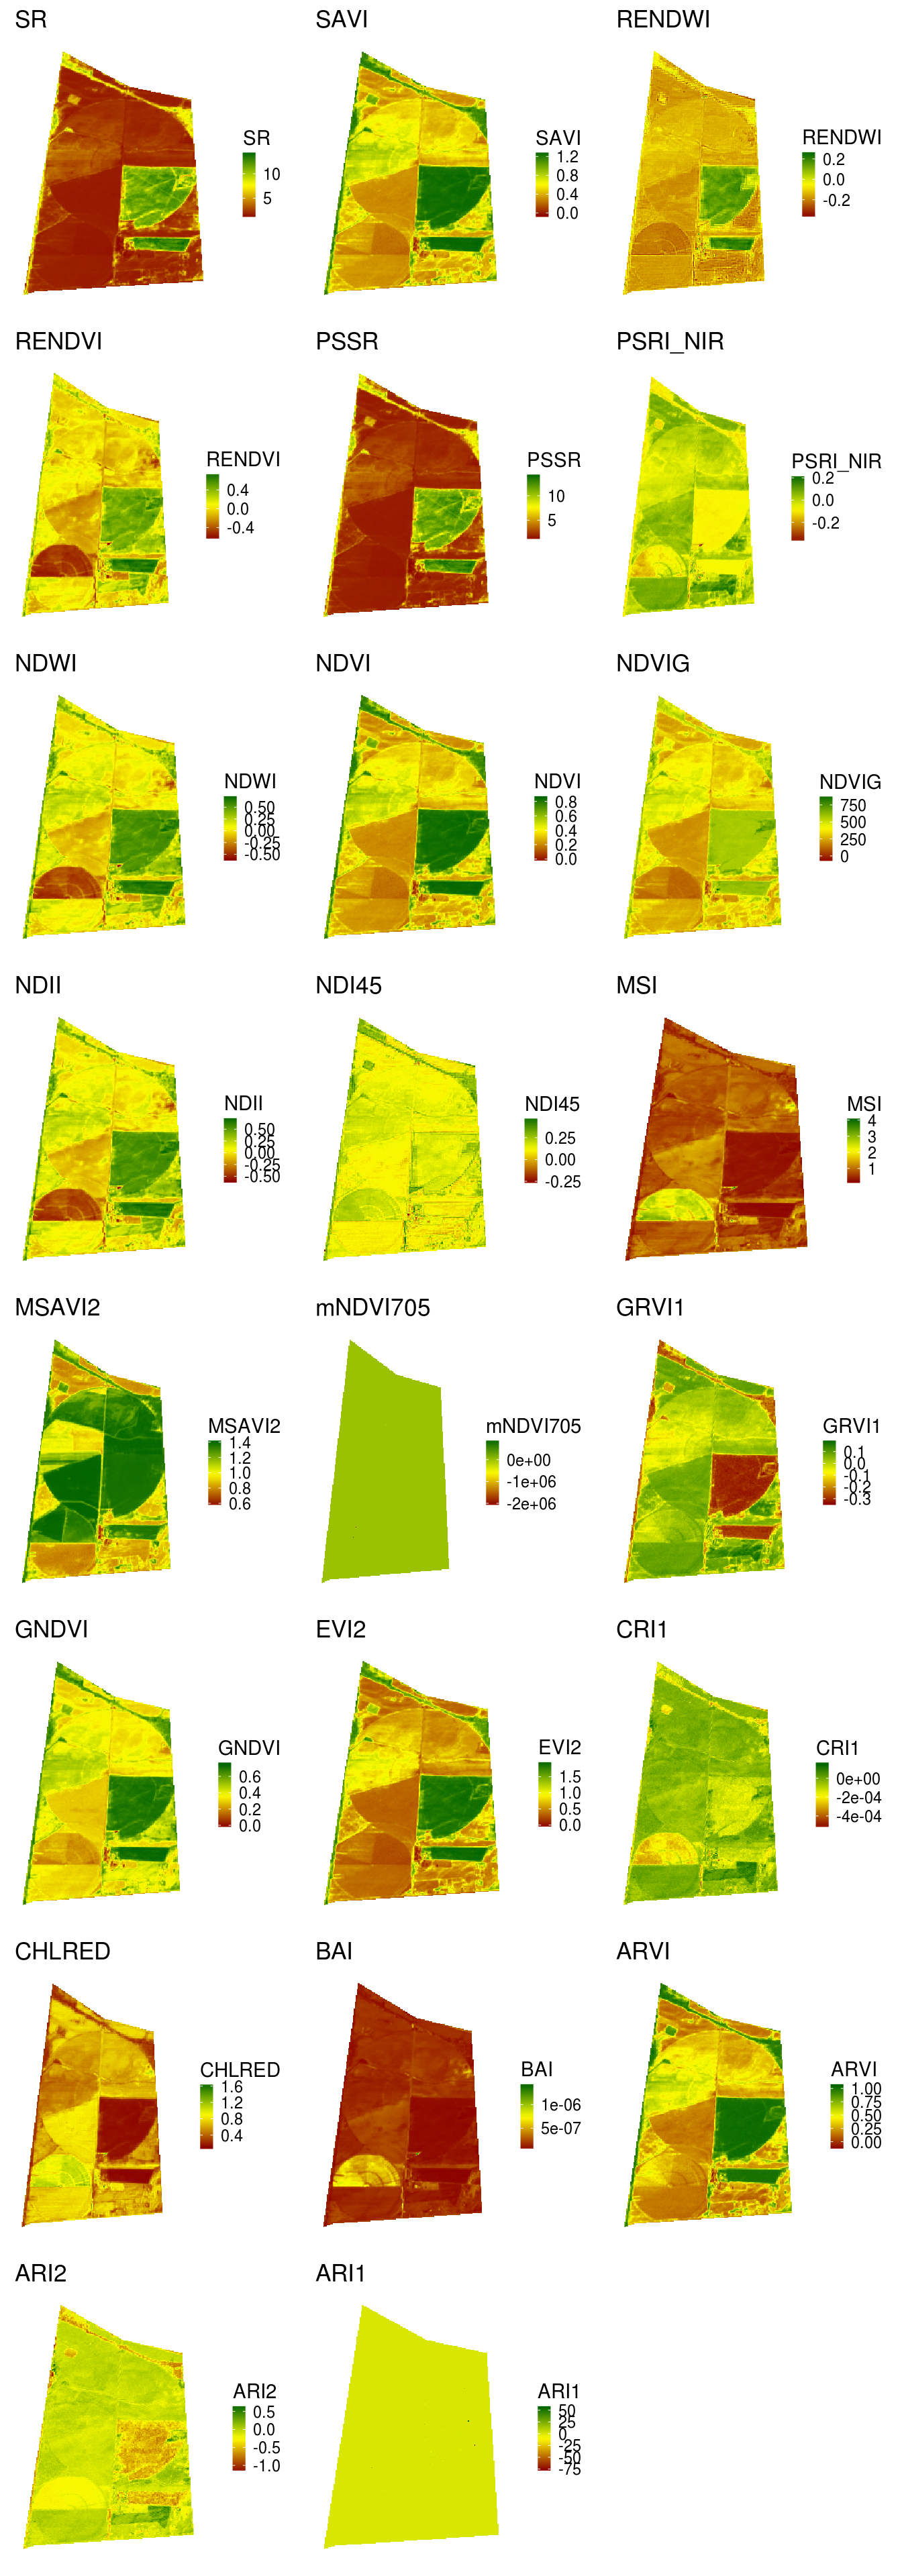
\includegraphics[width=1\linewidth]{bookdown-demo_files/figure-latex/Fron-1} 

}

\caption{Índices vegetacionales}\label{fig:Fron}
\end{figure}

\section{Predios Fernando Rueda}\label{predios-fernando-rueda-1}

\subsection{Predio 1}\label{predio-1-1}

\begin{figure}

{\centering 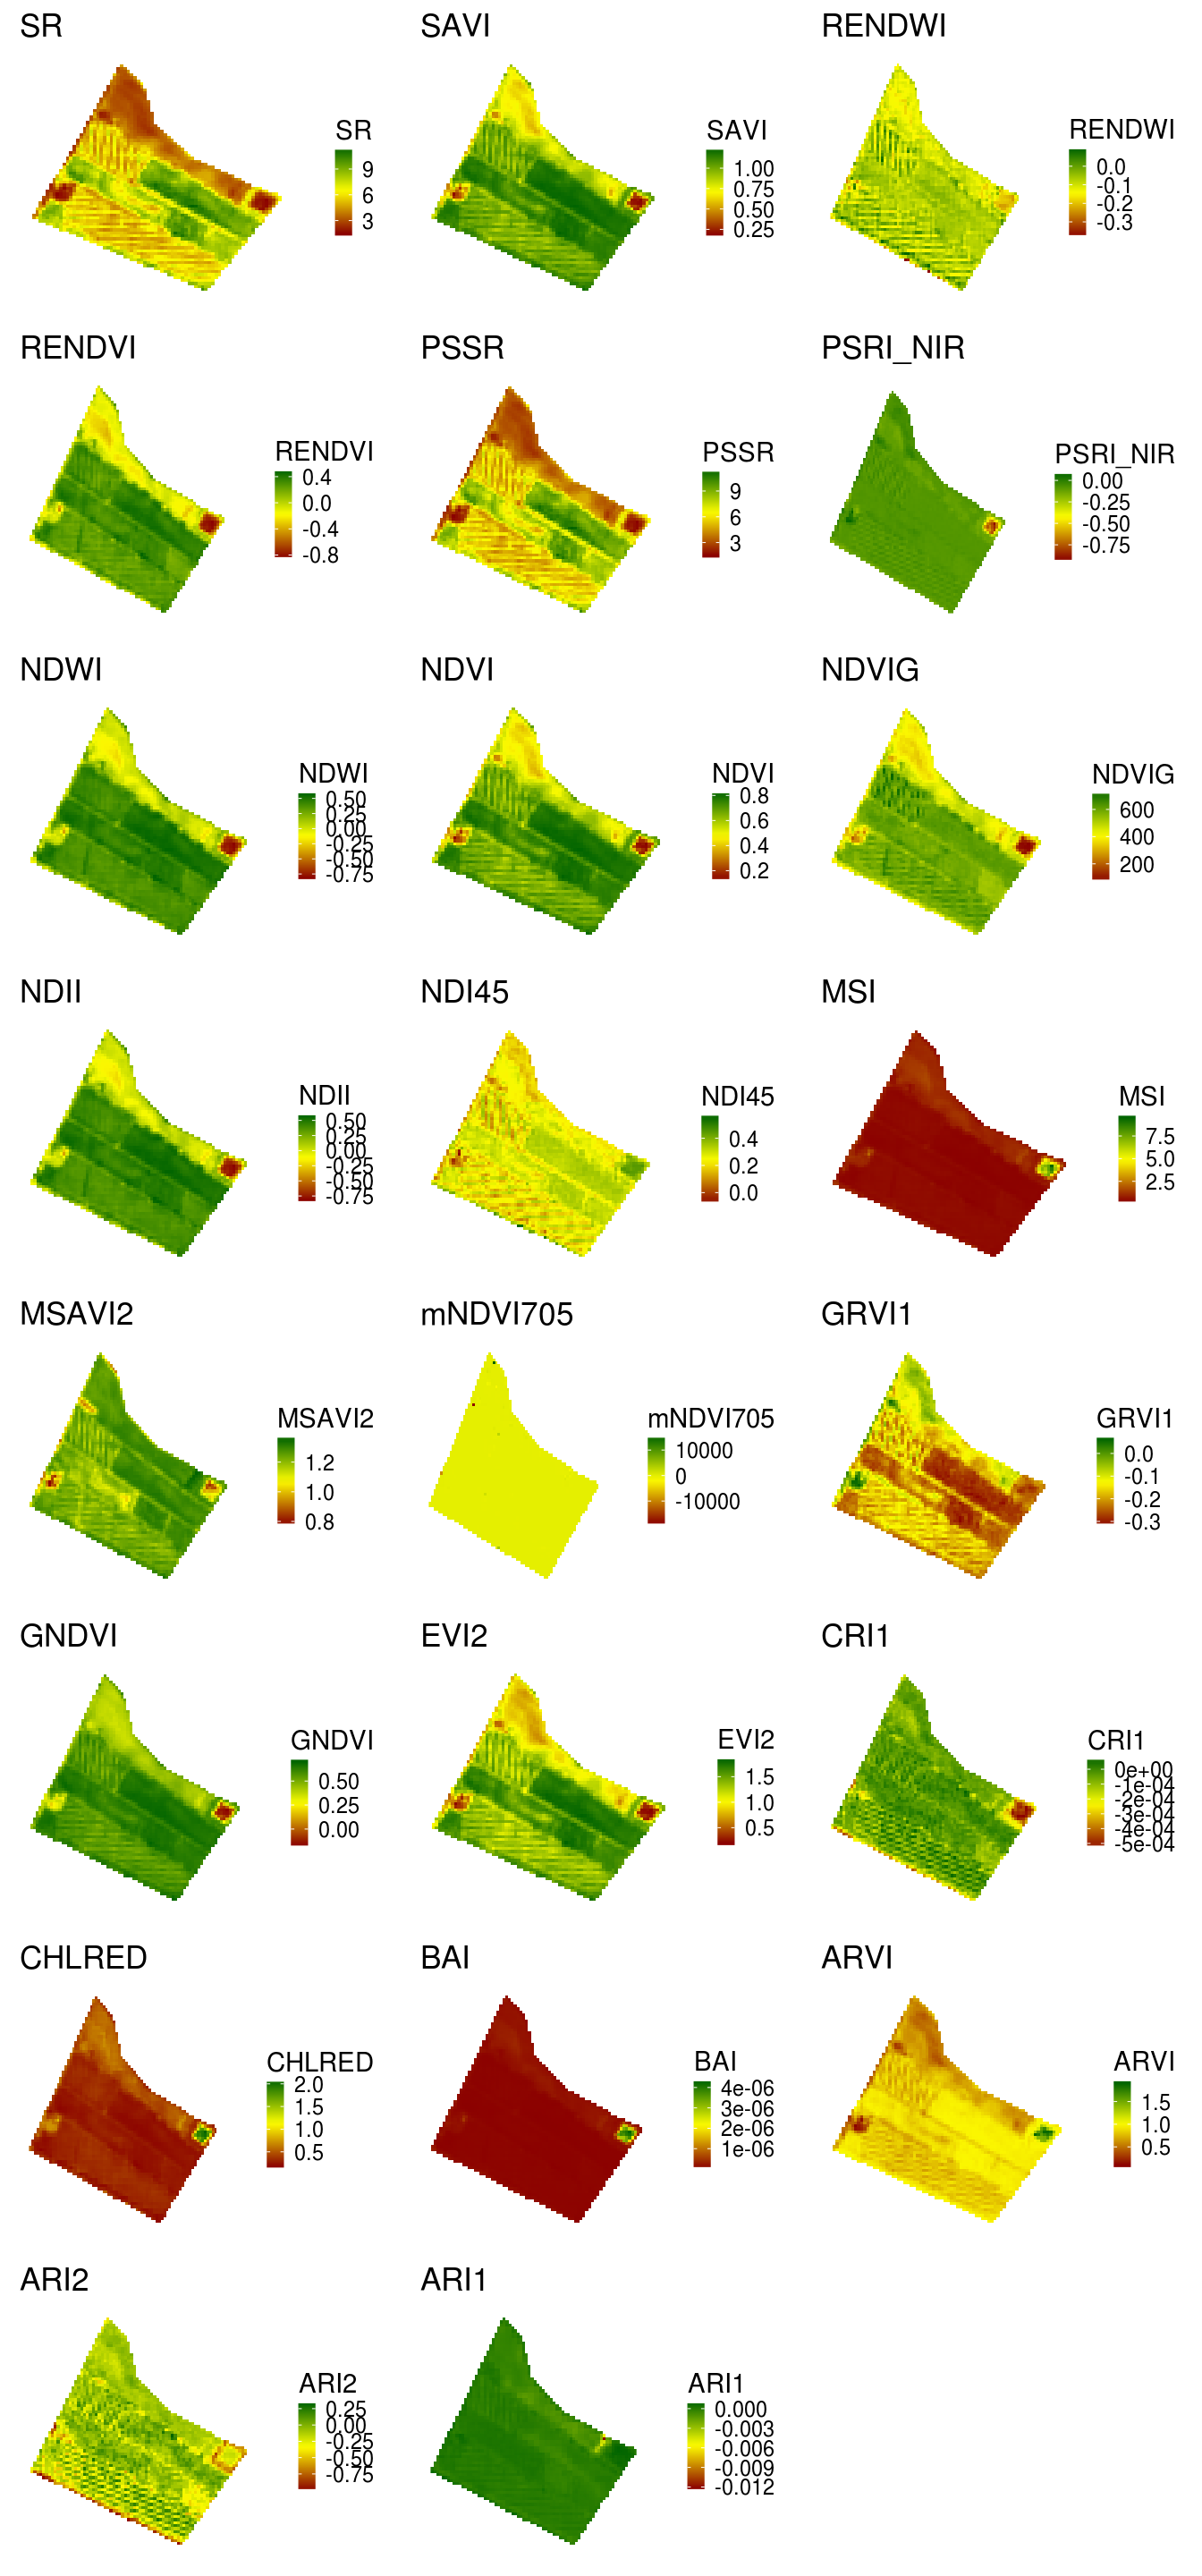
\includegraphics[width=1\linewidth]{bookdown-demo_files/figure-latex/FR1vis-1} 

}

\caption{Índices vegetacionales}\label{fig:FR1vis}
\end{figure}

\subsection{Predio 2}\label{predio-2-1}

\begin{figure}

{\centering 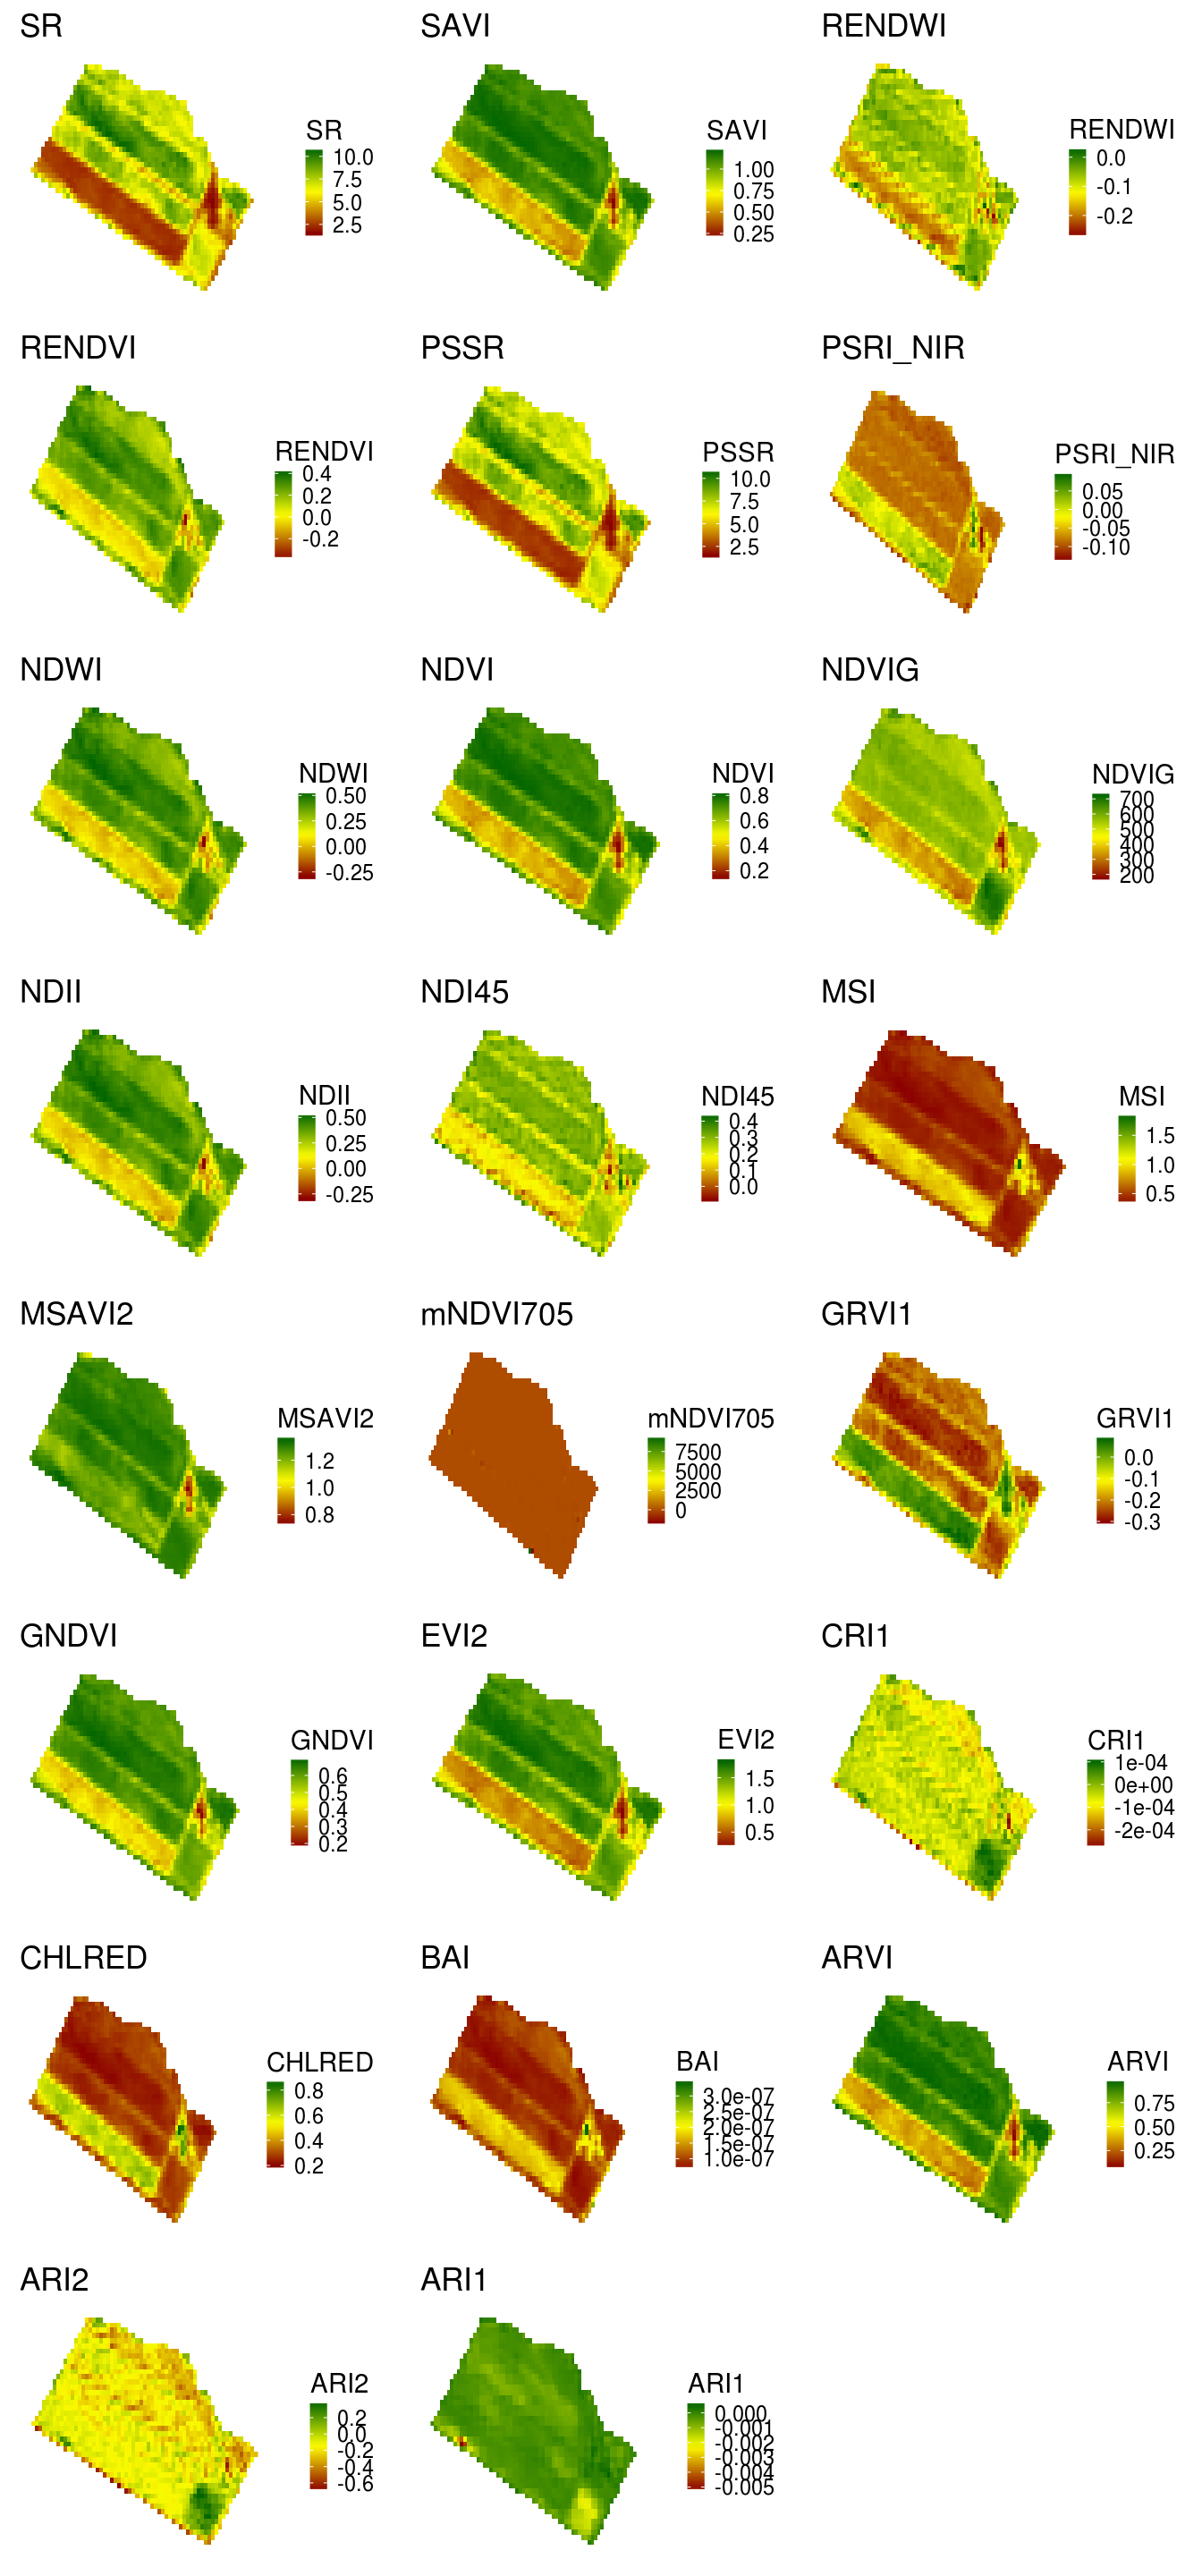
\includegraphics[width=1\linewidth]{bookdown-demo_files/figure-latex/FR2vis-1} 

}

\caption{Índices vegetacionales}\label{fig:FR2vis}
\end{figure}

\subsection{Predio 3}\label{predio-3-1}

\begin{figure}

{\centering 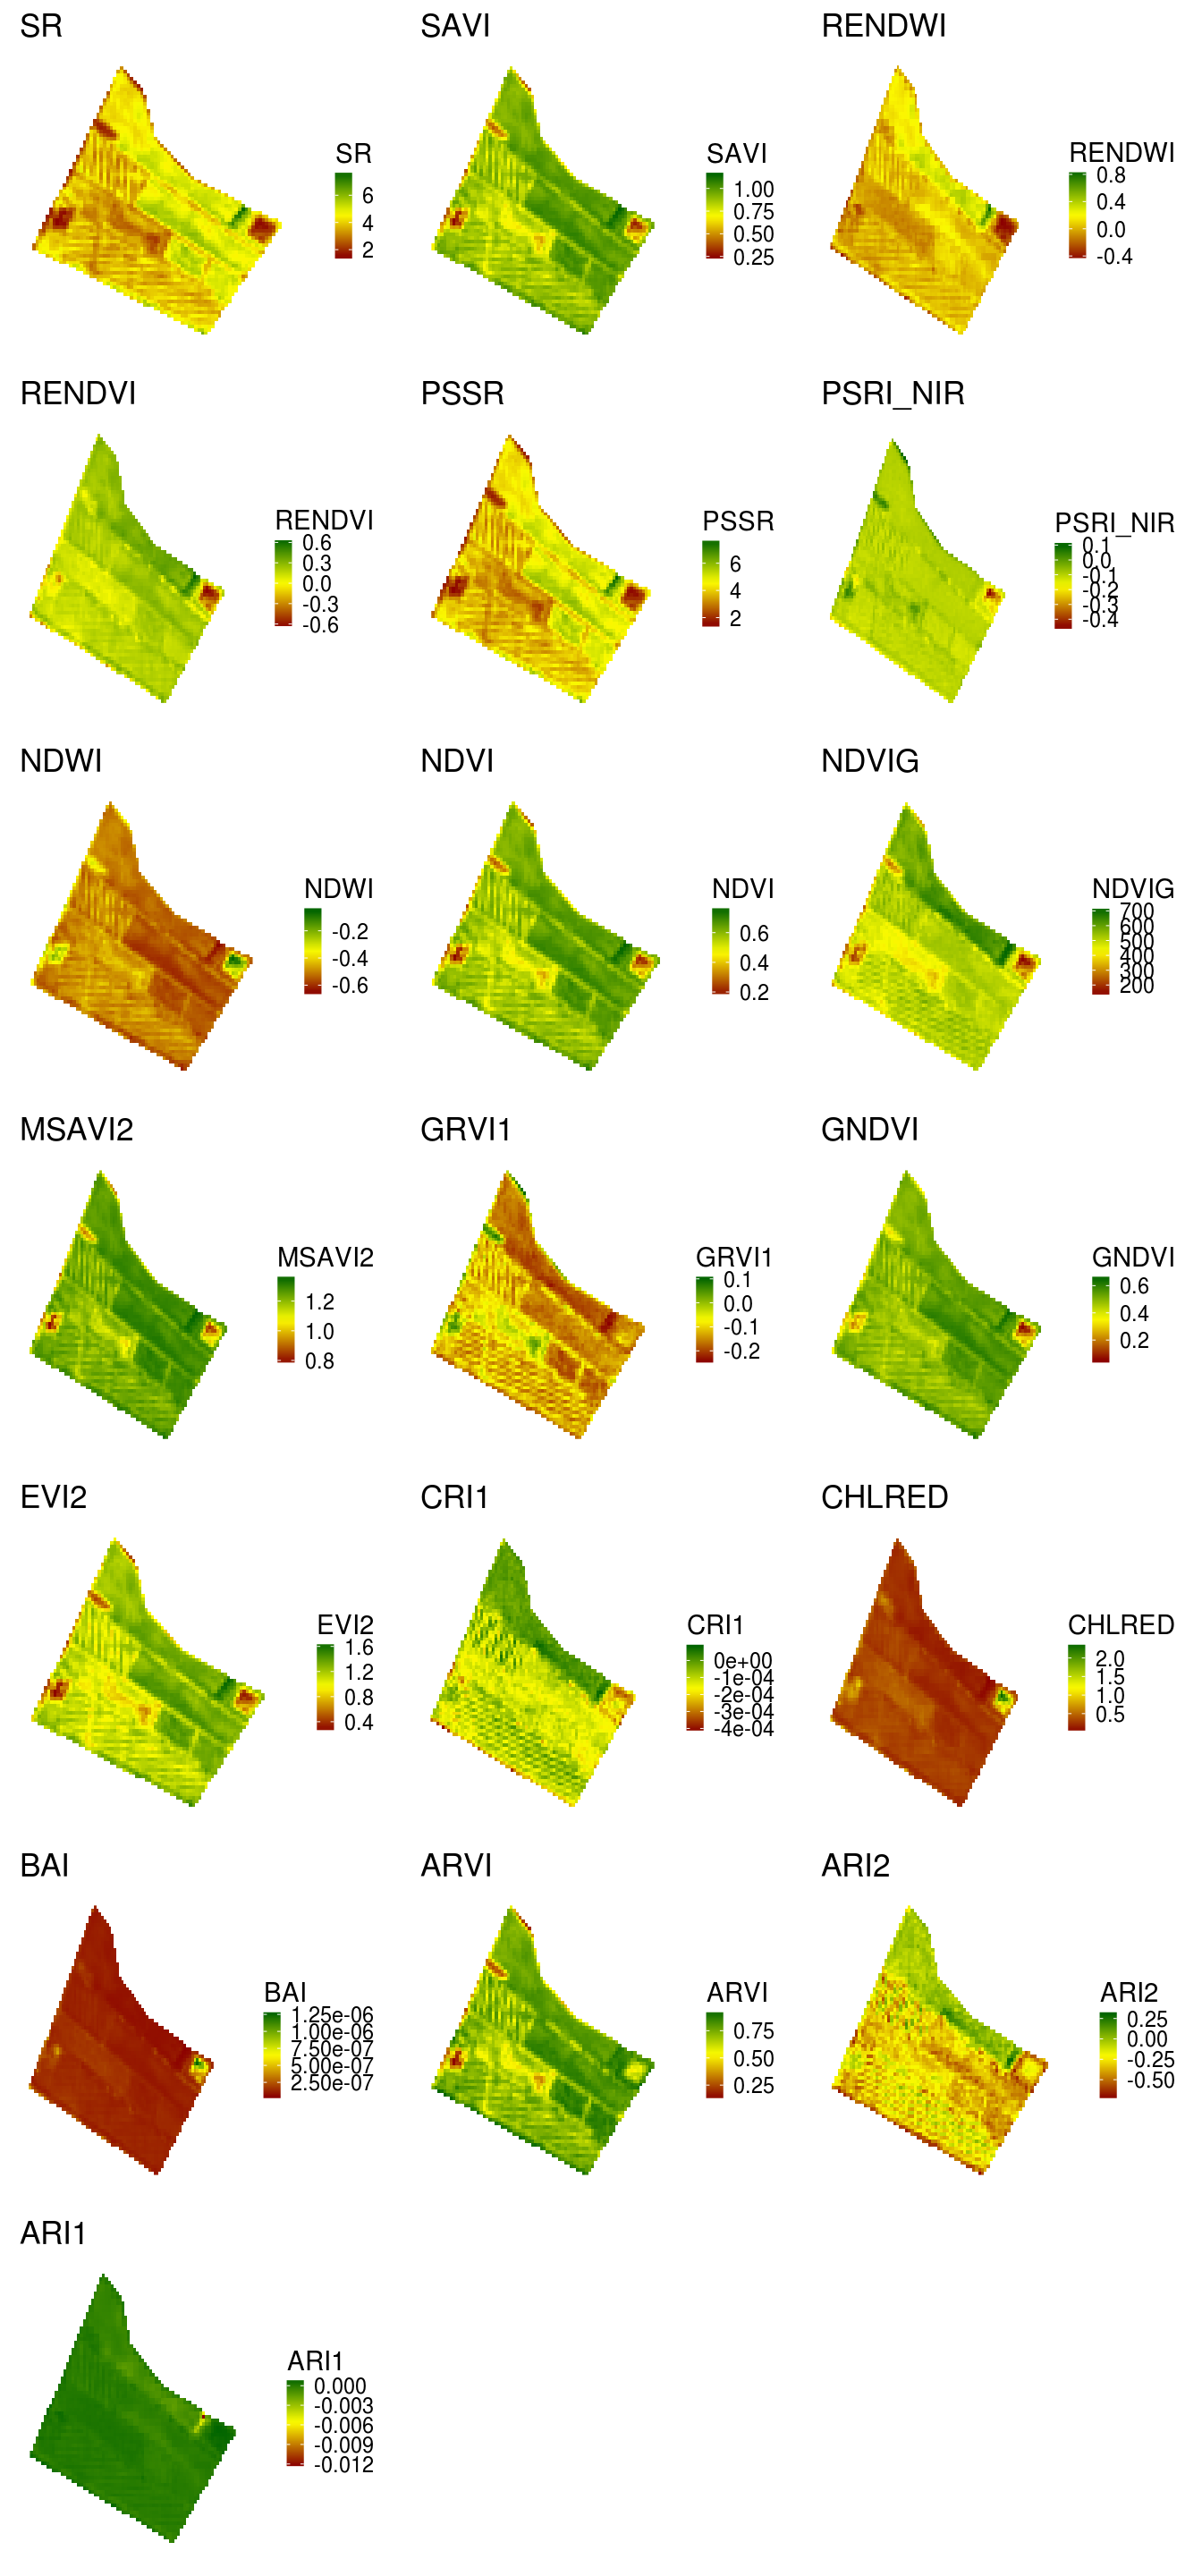
\includegraphics[width=1\linewidth]{bookdown-demo_files/figure-latex/FR3vis-1} 

}

\caption{Índices vegetacionales}\label{fig:FR3vis}
\end{figure}

\subsection{Predio 4}\label{predio-4-1}

\begin{figure}

{\centering 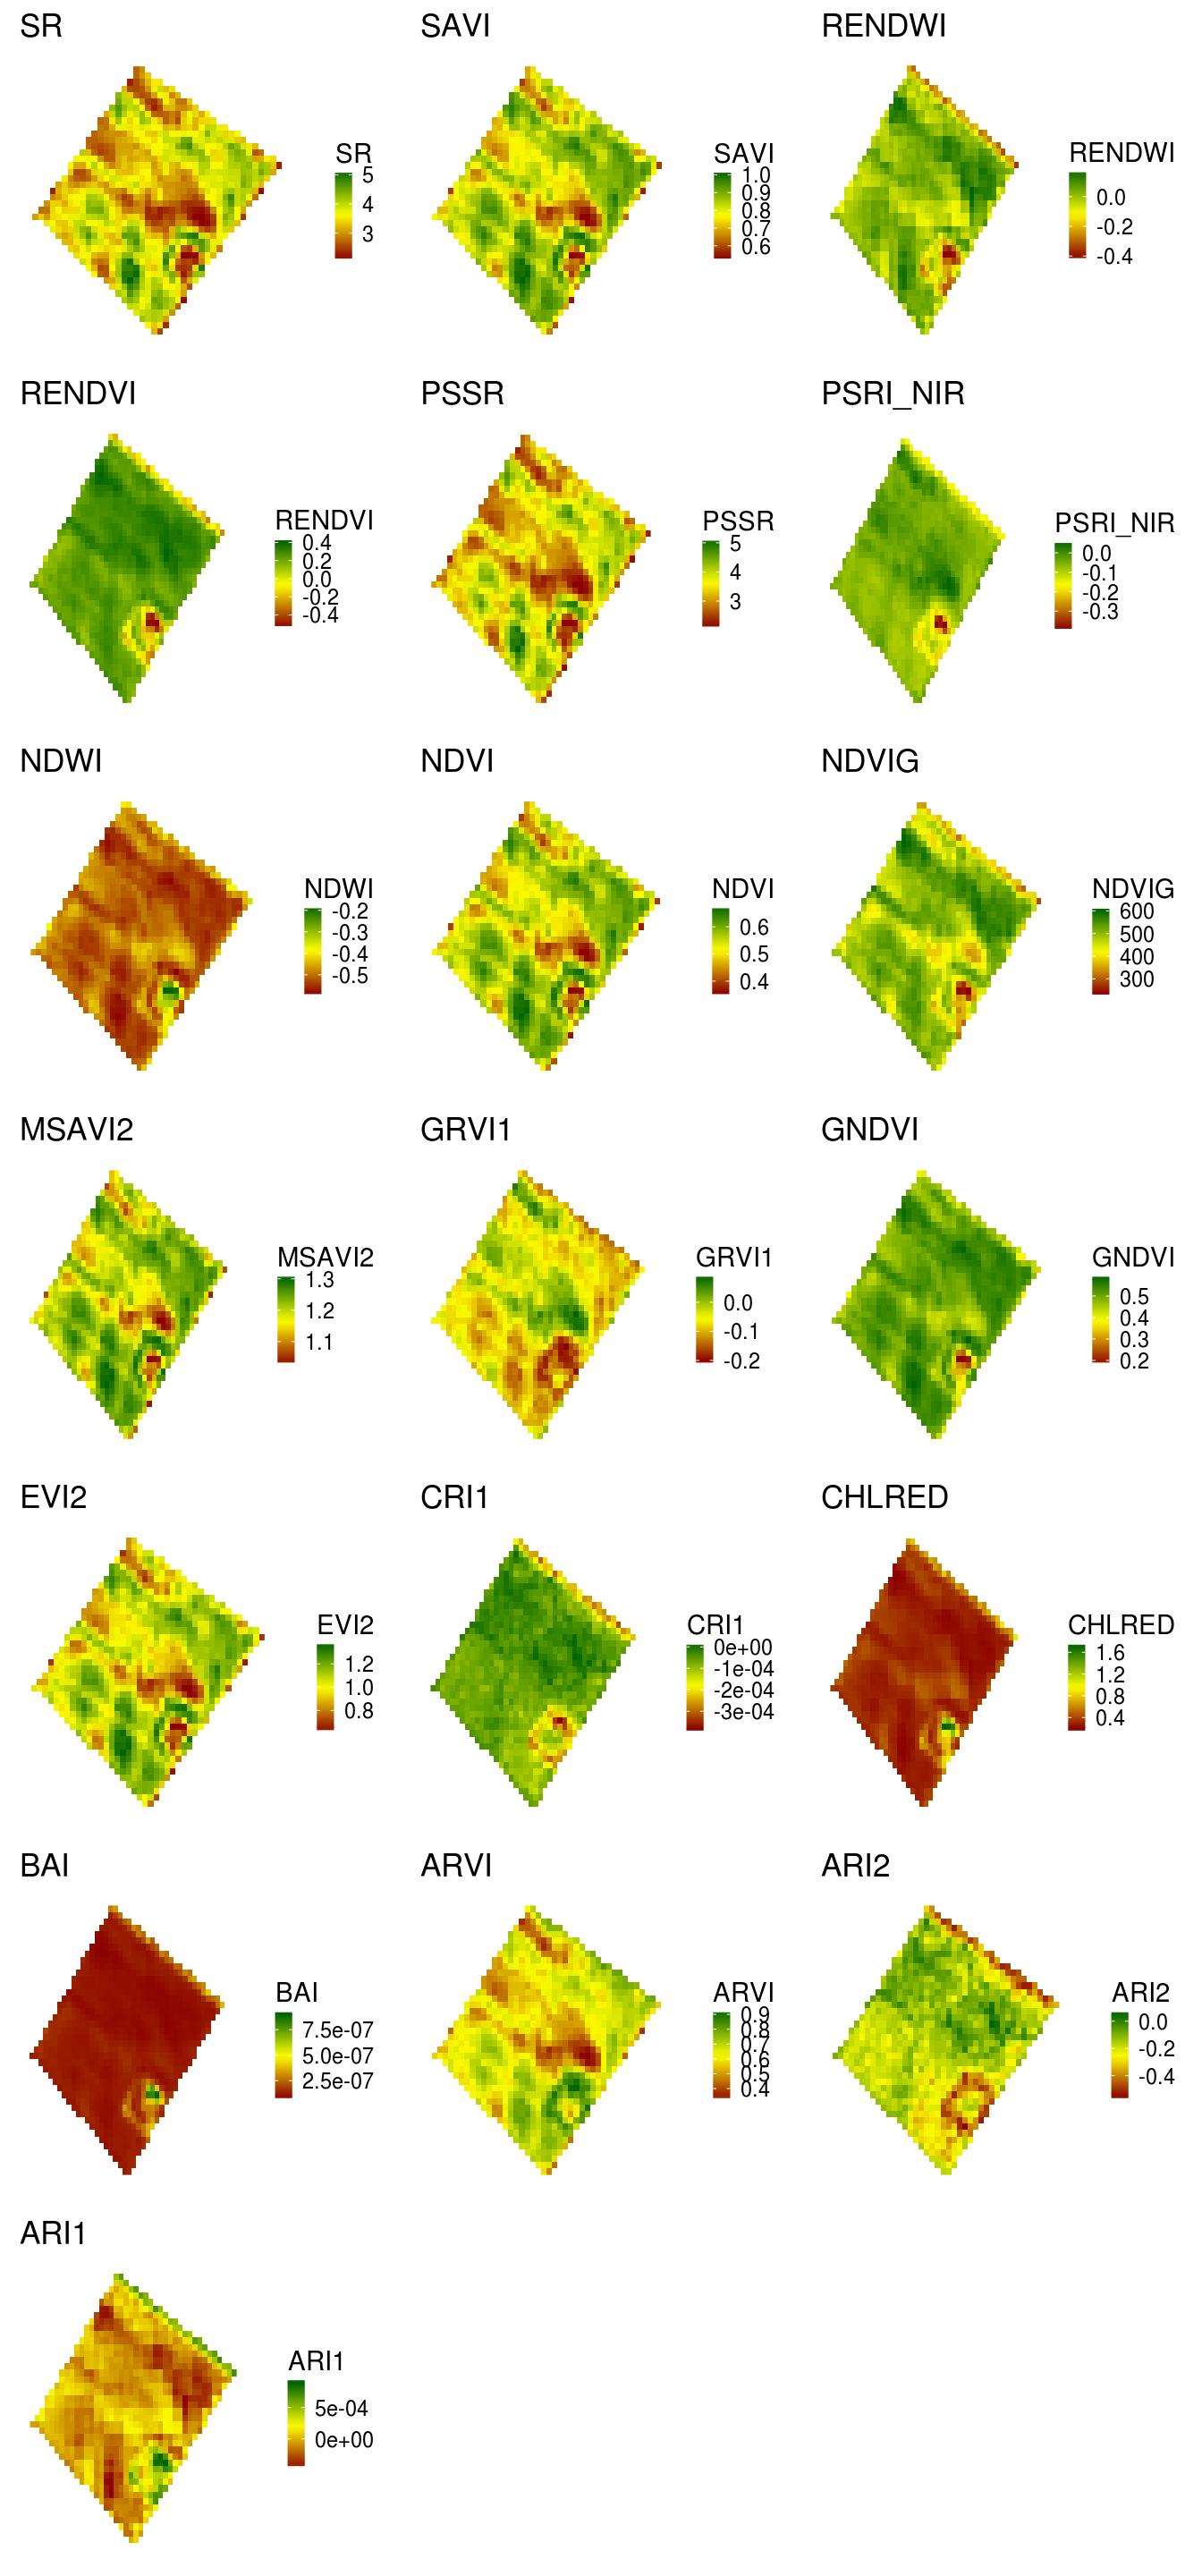
\includegraphics[width=1\linewidth]{bookdown-demo_files/figure-latex/FR4vis-1} 

}

\caption{Índices vegetacionales}\label{fig:FR4vis}
\end{figure}

\subsection{Predio 5}\label{predio-5-1}

\begin{figure}

{\centering 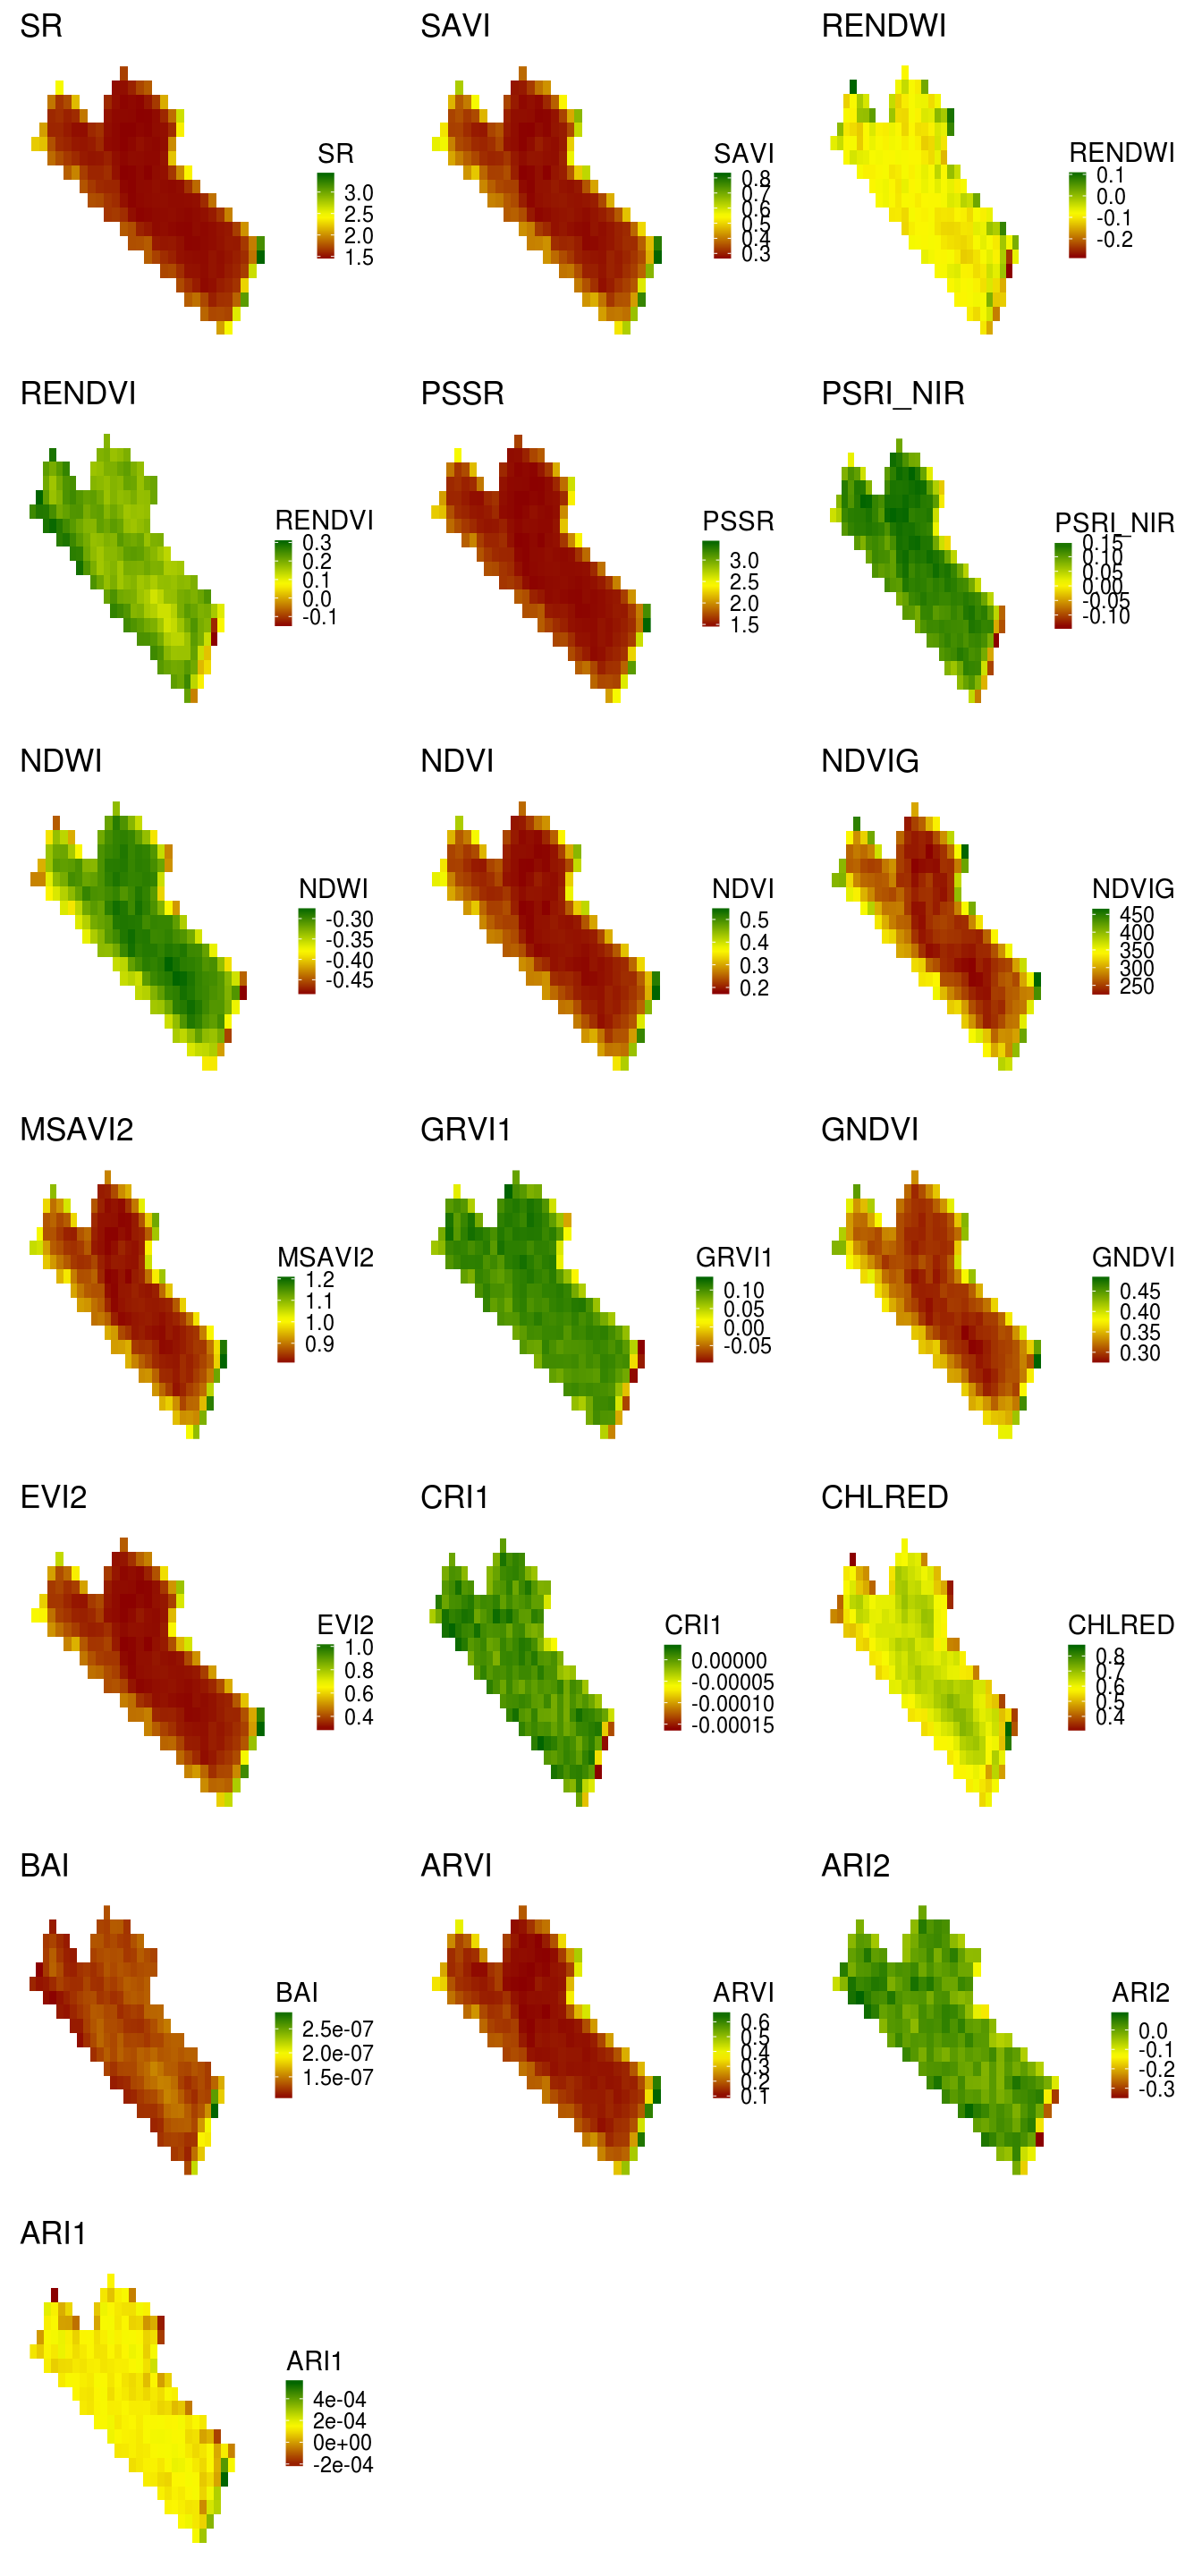
\includegraphics[width=1\linewidth]{bookdown-demo_files/figure-latex/FR5vis-1} 

}

\caption{Índices vegetacionales}\label{fig:FR5vis}
\end{figure}

\hypertarget{AnalisisDatos}{\chapter{Análisis de
Datos}\label{AnalisisDatos}}

En esta sección se presentan análisis simplificados derivados de los
índices vegetacionales usados,

\section{Fundo Rondadero}\label{fundo-rondadero-2}

\begin{figure}

{\centering \includegraphics[width=1\linewidth]{bookdown-demo_files/figure-latex/AnalisisFR-1} 

}

\caption{Índices vegetacionales}\label{fig:AnalisisFR}
\end{figure}

\section{Predios Fernando Rueda}\label{predios-fernando-rueda-2}

\subsection{Predio 1}\label{predio-1-2}

\begin{figure}

{\centering \includegraphics[width=1\linewidth]{bookdown-demo_files/figure-latex/AnalisisFR1-1} 

}

\caption{Índices vegetacionales}\label{fig:AnalisisFR1}
\end{figure}

\subsection{Predio 2}\label{predio-2-2}

\begin{figure}

{\centering \includegraphics[width=1\linewidth]{bookdown-demo_files/figure-latex/AnalisisFR2-1} 

}

\caption{Índices vegetacionales}\label{fig:AnalisisFR2}
\end{figure}

\subsection{Predio 3}\label{predio-3-2}

\begin{figure}

{\centering \includegraphics[width=1\linewidth]{bookdown-demo_files/figure-latex/AnalisisFR3-1} 

}

\caption{Índices vegetacionales}\label{fig:AnalisisFR3}
\end{figure}

\subsection{Predio 4}\label{predio-4-2}

\begin{figure}

{\centering \includegraphics[width=1\linewidth]{bookdown-demo_files/figure-latex/AnalisisFR4-1} 

}

\caption{Índices vegetacionales}\label{fig:AnalisisFR4}
\end{figure}

\subsection{Predio 5}\label{predio-5-2}

\begin{figure}

{\centering \includegraphics[width=1\linewidth]{bookdown-demo_files/figure-latex/AnalisisFR5-1} 

}

\caption{Índices vegetacionales}\label{fig:AnalisisFR5}
\end{figure}

\bibliography{packages.bib,book.bib}


\end{document}
